\documentclass[10pt,twocolumn]{article}

\usepackage[letterpaper,margin=0.75in,columnsep=0.28in]{geometry}
\usepackage[T1]{fontenc}
\usepackage{lmodern}
\usepackage{graphicx}
\usepackage{booktabs}
\usepackage{caption}
\usepackage{subcaption}
\usepackage{tikz}
\usetikzlibrary{shapes.geometric,arrows.meta,positioning,calc}
\usepackage{float}
\usepackage{amsmath}
\usepackage{amssymb}
\usepackage{microtype}
\usepackage[hidelinks]{hyperref}
\usepackage{titlesec}

\captionsetup{font=small,labelfont=bf}
\titlespacing*{\section}{0pt}{1.4ex plus .2ex}{0.6ex}
\titlespacing*{\subsection}{0pt}{1.0ex plus .2ex}{0.4ex}
\titleformat{\section}{\normalfont\large\bfseries}{\thesection}{0.6em}{}
\titleformat{\subsection}{\normalfont\normalsize\bfseries}{\thesubsection}{0.5em}{}
\setlength{\parskip}{0.15em}
\pagestyle{plain}

\newcommand{\yes}{\textbf{Y}}
\newcommand{\no}{N}

\begin{document}

\twocolumn[
\begin{@twocolumnfalse}
\begin{center}
{\LARGE\bfseries Tabletop Robot for Vision-Based\\[2pt]
Medication Verification at Home\par}
\vspace{0.8em}
{\large Nicole Cortes\par}
\vspace{0.2em}
{\normalsize M.S.\ Computer Science, Independent Study Final Paper\par}
\vspace{1.0em}
\begin{minipage}{0.86\textwidth}
\small
\textbf{Abstract.} Older adults who manage their own medication at home make
frequent errors. Polypharmacy, cognitive decline, and physical limits all play a
part. Most assistive technology only reminds people to take a dose. It does not
check that the pills in hand are the right ones. A review of 25 papers shows that no
prior study tests vision-based pill counting or verification on a real home robot.
This project asks whether a tabletop social robot (Reachy Mini) with a
vision-language model (VLM) can help with that verification step. We first tested
three VLMs on 15 controlled pill images using three prompts. Gemini was the most
accurate. Overlapping and touching pills were the main failure mode. Prompting on
its own did not fix counting errors. We then built a voice-conversational
verification system. It scans bottles, verifies doses, sets reminders, and checks
dose history. It also has safety rules that keep the robot inside the trust boundary
older adults prefer: it verifies and reminds, but it never gives clinical advice. A
four-route camera test (20 trials) shows that the system counts reliably except when
pills are dense and overlapping. That limit comes from the vision task itself, not
from the robot's camera or code path. We show three end-to-end interactions and
discuss the design, its limits, and future work.
\vspace{1.0em}
\end{minipage}
\end{center}
\end{@twocolumnfalse}
]

\section{Introduction}
Managing medication at home is one of the hardest parts of aging in place. Many
older adults take several medications on different schedules. This is called
polypharmacy. Cognitive decline makes it worse, especially decline in prospective
memory, which is the ability to remember to do something later
\cite{park1992,palen2006}. Physical limits like reduced dexterity and poor vision
also make it harder to handle pills and read labels \cite{pratiwi2023}. The most
common error is a missed dose. About 18\% of home-dwelling older adults miss at
least two doses per week, and 23\% report trouble remembering to take their
medications \cite{rantanen2017}. Adherence depends heavily on how much support a
person has. It runs from about 25\% in institutionalized patients with little help
to nearly 98\% in pharmacist-led programs \cite{mehany2026}. Non-adherence is
estimated to cost about \$100~billion per year in the United States
\cite{ansari2011}.

A lot of technology tries to help. This includes electronic pillboxes, smartphone
apps, smart dispensers, and dispensing robots. Most of it focuses on reminding the
user to take a dose. Very little of it checks that the pills about to be taken are
the right ones. Section~\ref{sec:related} goes through a review of 25 papers.
Computer vision for pill identification and counting shows up in only a few of them,
and none test those abilities on a real home robot. This project focuses on that
gap.

The main question is: Can a tabletop social robot, using a general-purpose
vision-language model, reliably support medication verification at home? This paper
makes the following contributions:
\begin{enumerate}\itemsep1pt
\item A controlled benchmark of three VLMs (ChatGPT, Claude, Gemini) on pill
counting across 15 images and three prompts (Section~\ref{sec:exp1}).
\item A prompting study that tests whether prompt engineering can fix VLM counting
errors (Section~\ref{sec:exp2}).
\item A working voice-conversational verification system on Reachy Mini. Its safety
rules follow the trust preferences reported in the literature
(Section~\ref{sec:system}).
\item A four-route camera comparison test that shows where counts break in the full
system (Section~\ref{sec:e2e}).
\item Three demonstrated end-to-end interactions (Section~\ref{sec:demo}).
\end{enumerate}

\section{Related Work}\label{sec:related}
\textbf{Pillboxes and organizers} are the most studied category. One review
catalogued 17 electronic pillbox systems, from simple organizers to devices with
alarms and locking. It found that many are poorly designed for older adults
\cite{miguel2018}. \textbf{Smart dispensing systems} add real-time tracking and
cloud syncing. A scoping review found 114 smart adherence products, about 70\% of
them already on the market \cite{faisal2023}. \textbf{Robotic dispensers} are the
closest prior work. The Evondos~E300 is a Class~I medical device in the EU. It hands
out pre-packaged sachets on schedule and reached 98.7\% on-time dose delivery in
homes \cite{rantanen2017}. It works well, but it only handles pre-packaged
medication and does not verify loose pills. \textbf{Apps} such as ALICE let patients
view images of their medications and get interaction warnings. In that study 88\% of
users reported feeling more independent \cite{consort2014}. \textbf{Ambient
displays} use indirect cues instead of explicit alarms. One study raised adherence
from 81\% to 96\% during the intervention. It then dropped to 77\% after the
technology was removed \cite{zarate2019}. That drop is a warning about technology
dependence. \textbf{AI methods} include reinforcement-learning reminder
personalization, deep networks with OCR for container identification, and NLP for
drug-drug interaction detection \cite{ciampi2022}.

Two findings guided the design. First, trust is task-specific. Older adults are fine
with robots handling reminders, but they want humans to make medication decisions
\cite{prakash2013}. Second, the best systems share a few design principles. They use
multi-modal cues (audio and visual), large fonts, caregiver integration, fail-safe
escalation, and personalization that respects existing routines
\cite{rantanen2017,miguel2018,palen2006}. We found no study that tests vision-based
pill counting on a home robot. That is the contribution of this work.

\section{Experiment 1: VLM Model Comparison}\label{sec:exp1}
\textbf{Goal.} Find which general-purpose VLM counts pills most reliably, and find
the conditions that make counting fail.

\textbf{Method.} We built 15 pill images. The true counts were 3, 5, 7, 10, and 15.
The images covered a set of difficulty variables: baseline, spacing, touching,
overlapping, background clutter, lighting, shadows, color contrast, and color
uniformity. We sent each image to three models: OpenAI ChatGPT, Anthropic Claude,
and Google Gemini. We used three prompts for each one. The first was a naive prompt
(``How many pills are in this image?''). The second was a careful chain-of-thought
prompt (``count each visible pill systematically''). The third was a
self-verification prompt (``after you answer, double-check by counting again and
confirm or correct''). For each trial we recorded the model's count, the signed
error, and whether it matched ground truth.

\textbf{Results.} Table~\ref{tab:exp1} shows accuracy and mean absolute error (MAE)
by model and prompt. Gemini was the clear winner. It was near-perfect across all
three prompts, and its only errors were on overlapping pills. Claude did well on
separated pills but undercounted badly when pills touched or overlapped (off by 3 to
4). ChatGPT got worse at high counts (15) and on low-contrast images. Background and
lighting mattered much less than expected.

\begin{table}[H]
\centering
\caption{Experiment 1: pill-counting accuracy (\% correct, $n{=}15$) and mean
absolute error (MAE, pills) by model and prompt. P1 = naive, P2 = careful,
P3 = double-check.}
\label{tab:exp1}
\small
\begin{tabular}{@{}lccccc@{}}
\toprule
& \multicolumn{3}{c}{Accuracy} & \multicolumn{2}{c}{MAE}\\
\cmidrule(lr){2-4}\cmidrule(lr){5-6}
Model & P1 & P2 & P3 & Overall & Overall\\
\midrule
ChatGPT & 60\% & 53\% & 73\% & 62\% & 0.44\\
Claude  & 73\% & 73\% & 73\% & 73\% & 0.51\\
\textbf{Gemini}  & \textbf{93\%} & \textbf{100\%} & \textbf{93\%} & \textbf{96\%} & \textbf{0.04}\\
\bottomrule
\end{tabular}
\end{table}

\textbf{Key finding.} Two things drive counting reliability: the choice of model and
the physical arrangement of the pills, mainly whether they touch or overlap. Surface
image properties matter less. This is why we used Gemini as the production backend
(Section~\ref{sec:system}).

\section{Experiment 2: Does Prompting Fix Errors?}\label{sec:exp2}
Once we knew Gemini was the best model, we tested whether prompt engineering could
push accuracy higher. We ran ten prompting strategies on Gemini. They ranged from a
naive baseline to color-first decomposition, bounding-box detection, spatial
partitioning, an uncertainty-aware medication-safety persona, and a
Set-of-Mark-style numbered-labeling prompt.

The result was mostly negative. Prompting did not reliably fix counting errors. When
a model miscounted, asking it to ``double-check'' or to ``go through systematically''
usually gave the same wrong number again. The reasoning was more structured and more
confident, but the answer did not change. The one promising direction in our notes
was decomposition by color subgroup. Breaking the count into smaller groups of one
color seems to reduce estimation error. The practical takeaway is that better
hard-case accuracy depends more on what the model sees, such as capture quality and
spreading the pills out, than on how it is asked.

\section{System Design}\label{sec:system}
\textbf{Architecture.} The system builds on a conversational Reachy Mini
application. A real-time voice model handles speech. The robot's head-mounted camera
provides vision. Gemini does all label reading and pill counting. A lightweight
in-memory store holds the saved medications and a dose log. A web UI mirrors the
interaction. Figure~\ref{fig:flow} shows the medication workflow in five phases.

\begin{figure}[H]
\centering
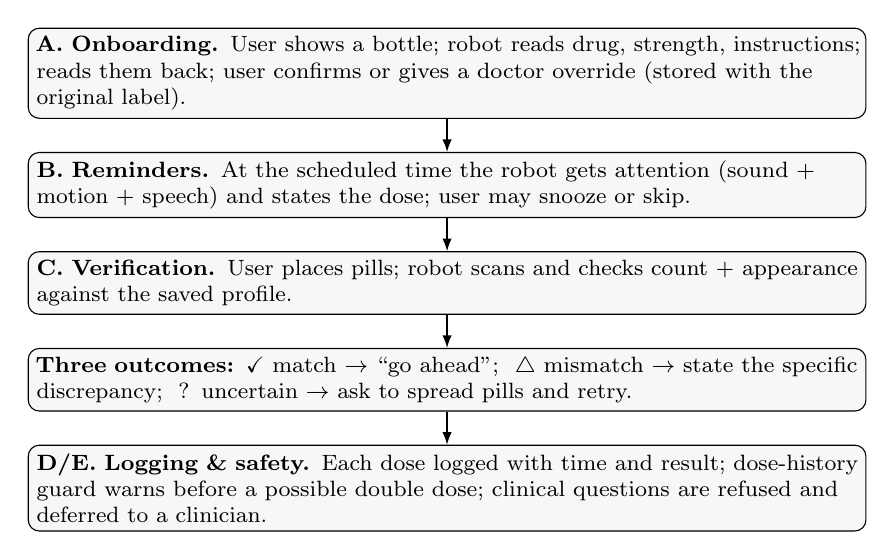
\begin{tikzpicture}[
  node distance=4.2mm,
  box/.style={rectangle,rounded corners,draw,line width=0.4pt,
    text width=0.86\columnwidth,align=left,inner sep=3pt,font=\footnotesize,fill=black!3},
  lbl/.style={font=\footnotesize\bfseries},
  arr/.style={-{Latex[length=1.6mm]},line width=0.5pt}
]
\node[box] (a) {\textbf{A. Onboarding.} User shows a bottle; robot reads drug,
strength, instructions; reads them back; user confirms or gives a doctor override
(stored with the original label).};
\node[box,below=of a] (b) {\textbf{B. Reminders.} At the scheduled time the robot
gets attention (sound + motion + speech) and states the dose; user may snooze or
skip.};
\node[box,below=of b] (c) {\textbf{C. Verification.} User places pills; robot scans
and checks count + appearance against the saved profile.};
\node[box,below=of c] (d) {\textbf{Three outcomes:} \checkmark\ match $\rightarrow$
``go ahead'';\ \ $\triangle$ mismatch $\rightarrow$ state the specific discrepancy;\ \
? uncertain $\rightarrow$ ask to spread pills and retry.};
\node[box,below=of d] (e) {\textbf{D/E. Logging \& safety.} Each dose logged with
time and result; dose-history guard warns before a possible double dose; clinical
questions are refused and deferred to a clinician.};
\draw[arr] (a) -- (b);
\draw[arr] (b) -- (c);
\draw[arr] (c) -- (d);
\draw[arr] (d) -- (e);
\end{tikzpicture}
\caption{Medication workflow. The robot verifies and reminds but never makes a
medication decision, keeping it inside the trust boundary older adults prefer
\cite{prakash2013}.}
\label{fig:flow}
\end{figure}

\textbf{Design choices from the literature.} The system follows the design
principles from Section~\ref{sec:related}. (i) It uses multi-modal cues (speech,
head motion, and a screen) for reminders. (ii) It has a fail-safe three-way
verification outcome, so the robot never confidently confirms a bad count. (iii) It
handles doctor overrides directly. It stores the change next to the original printed
label and flags it. (iv) It keeps trust-aware task boundaries. The robot reads
labels, counts pills, compares against saved profiles, and reminds the user. It is
not allowed to give medical advice, recommend dosage changes, or answer interaction
questions. A dose-history check warns the user when a medication is already logged as
taken. This guards against an accidental double dose.

\textbf{One important engineering decision.} An early version of the code used
whichever VLM API key was present. In practice that selected Claude, the worst
performer on overlapping pills in Experiment~1. We forced the backend to Gemini, the
best model in our tests. This was a one-line change, but it had a large effect on
real-world accuracy. It also shows why running the benchmark before the build
mattered.

\section{End-to-End Evaluation: Camera Comparison Test}\label{sec:e2e}
\textbf{Goal.} Clean photos counted well in Experiment~1, but the robot still
miscounted sometimes in daily use. We designed a test to find where the error comes
from: the model, the captured photo, or the code path.

\textbf{Method.} We used four pill setups: Easy, Medium, Hard, and a denser
Hard-Closer / Hard-No-Overlap variant. For each setup we ran the same arrangement
through four routes. Route (A) was a clean phone photo sent straight to Gemini.
Route (B) was that same photo sent through the robot's own code path. Route (C) was
the robot's three captured snapshots sent to Gemini. Route (D) was the full robot
scan from start to finish. We kept the arrangement fixed across routes, so any
change in the answer points to one stage. Figure~\ref{fig:views} shows the robot's
view of an easy and a hard arrangement.

\begin{figure}[H]
\centering
\begin{subfigure}{0.49\columnwidth}
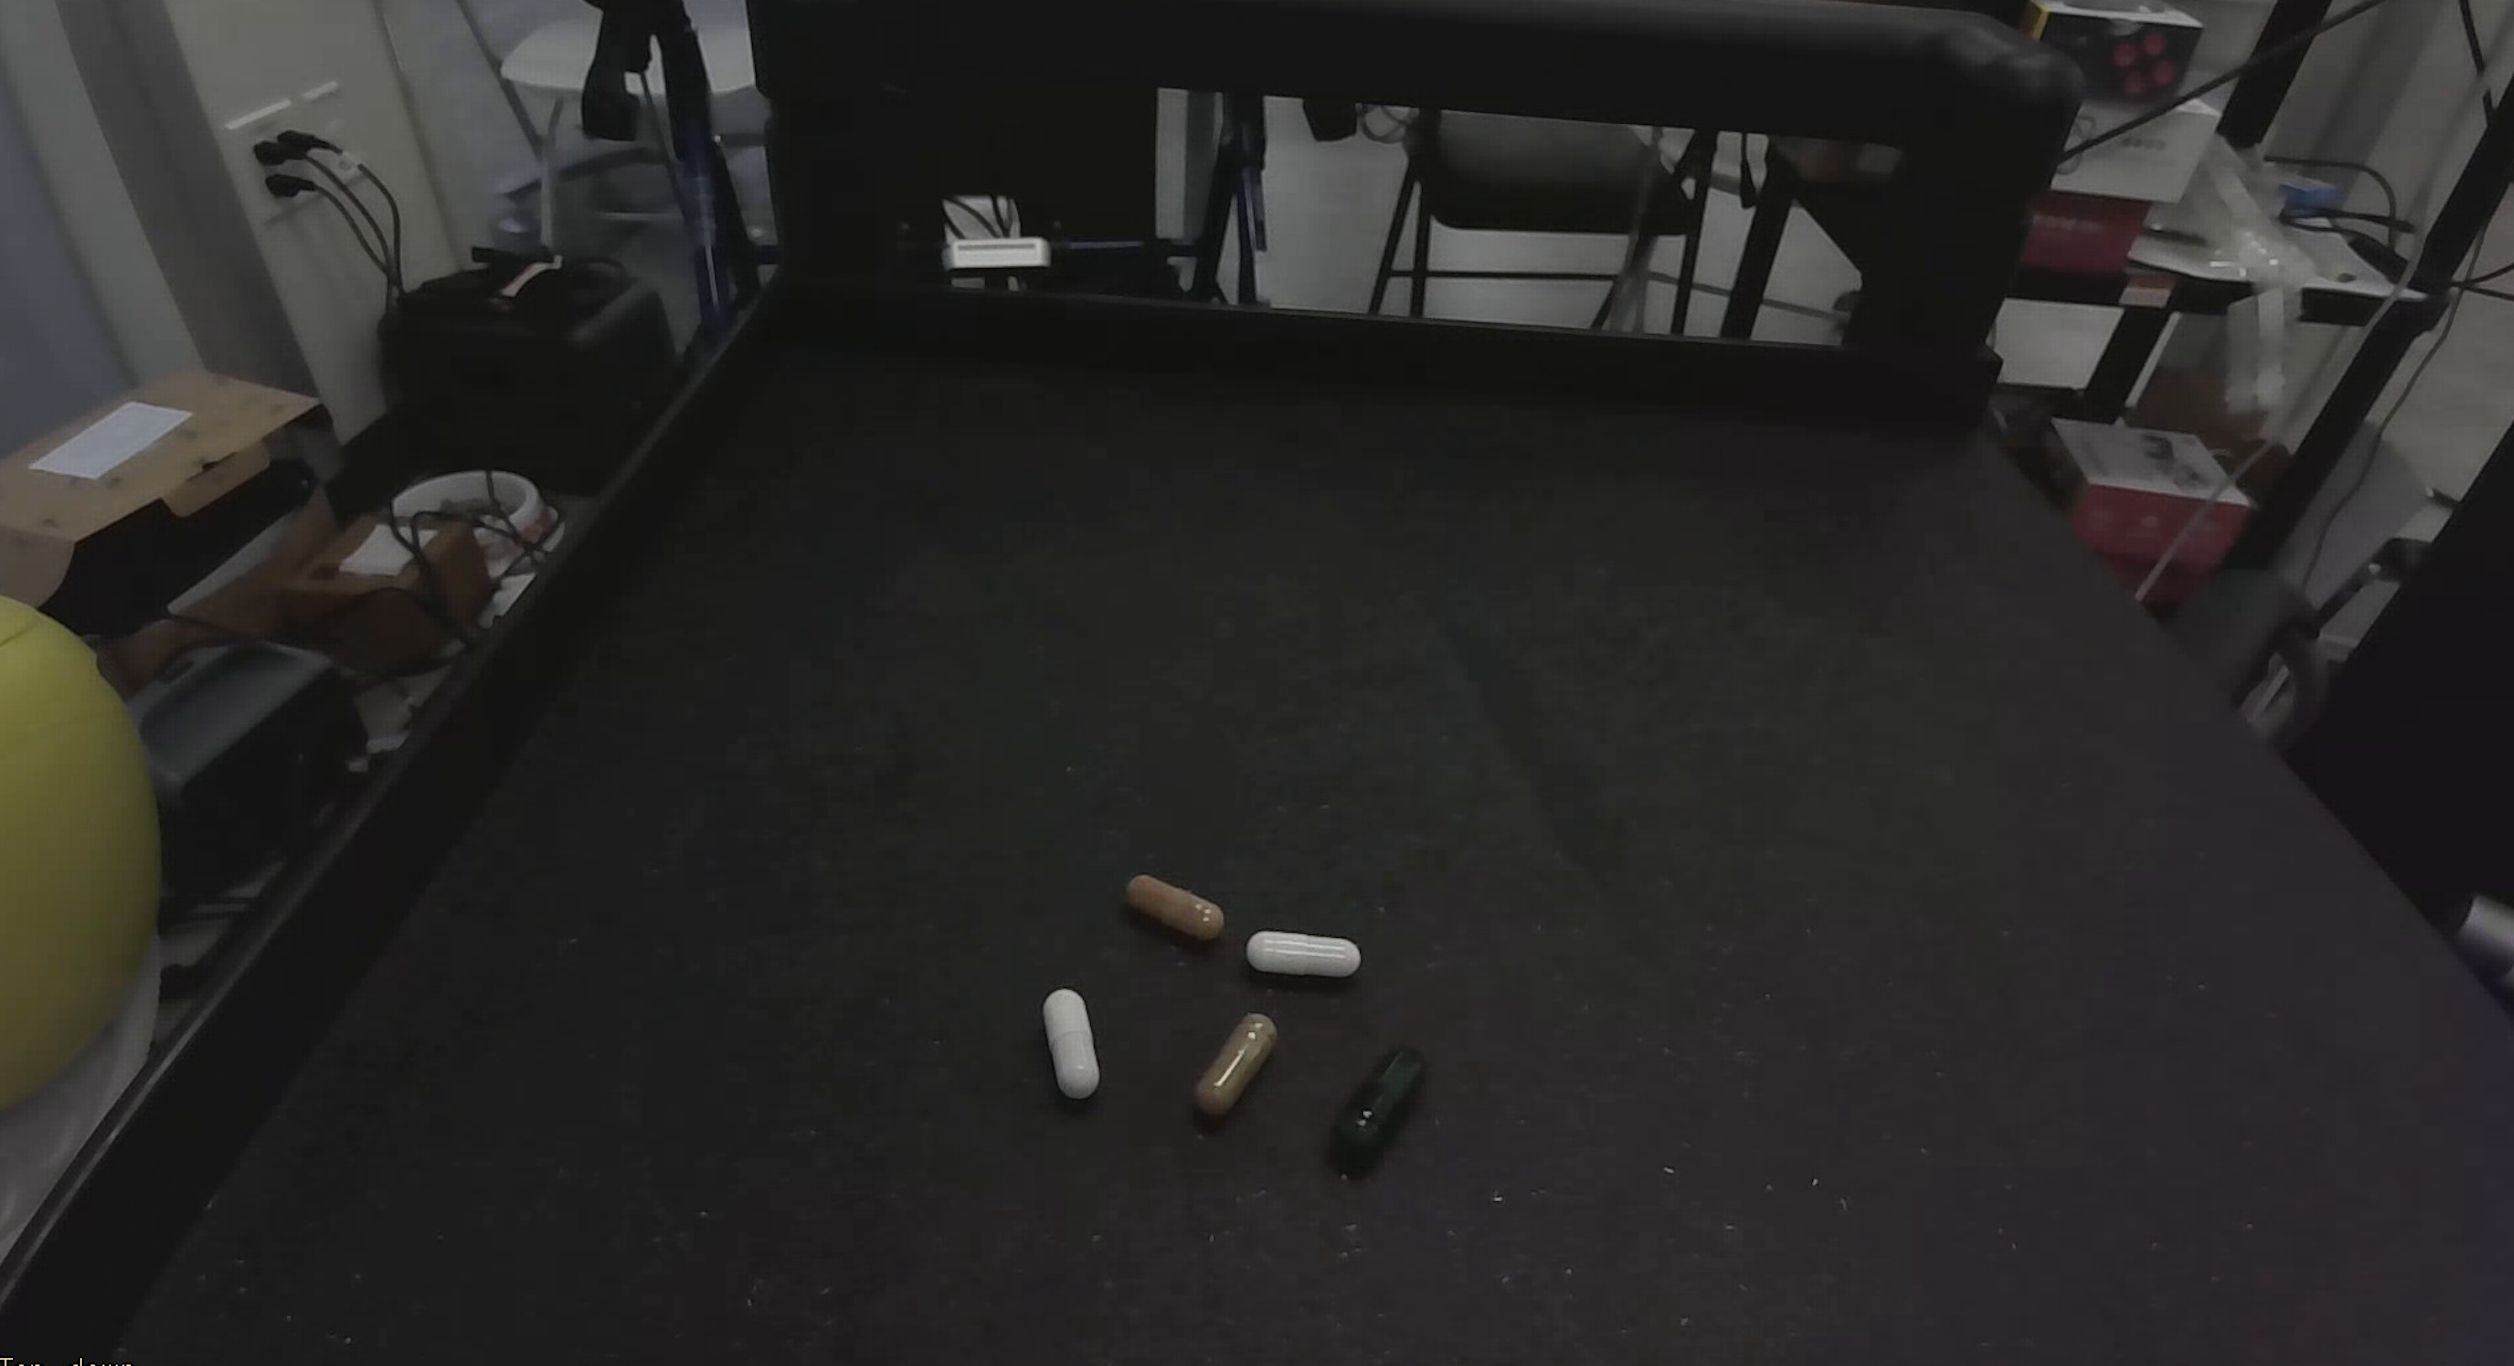
\includegraphics[width=\linewidth]{figures/easy_view.png}
\caption{Easy: 5 separated}
\end{subfigure}\hfill
\begin{subfigure}{0.49\columnwidth}
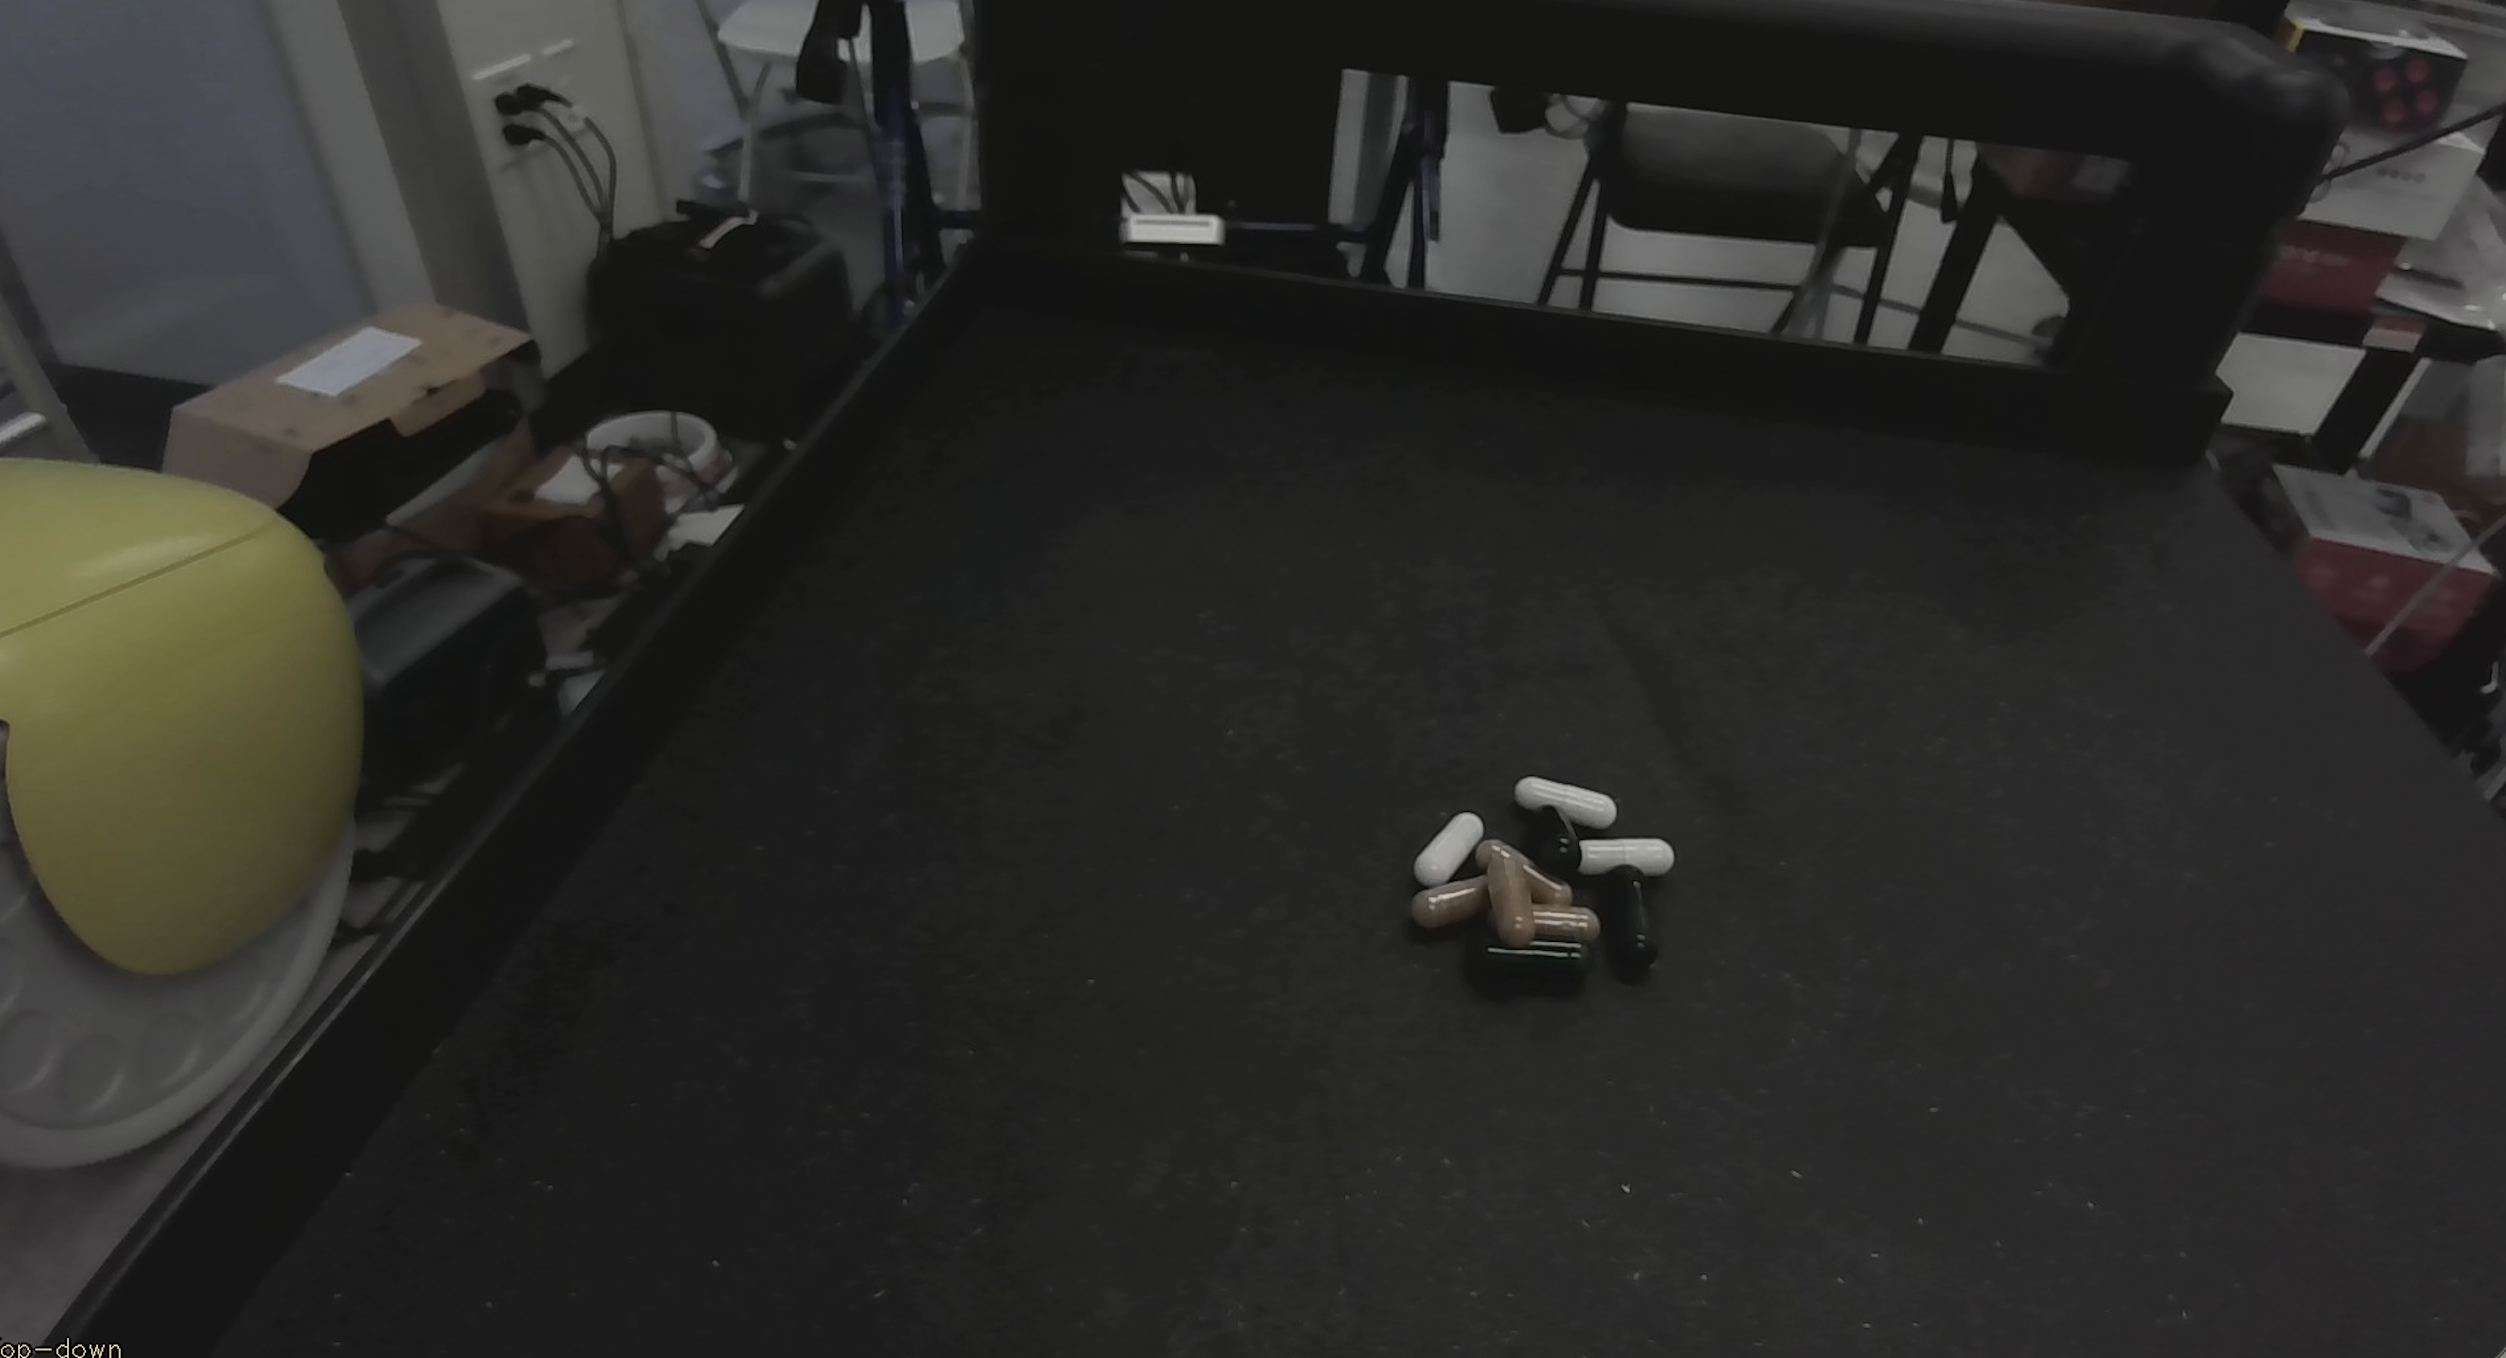
\includegraphics[width=\linewidth]{figures/hard_view.png}
\caption{Hard: overlapping}
\end{subfigure}
\caption{Reachy Mini's camera view. Separated pills (a) are counted reliably across
all routes; clustered, overlapping pills (b) are where every miscount occurred.}
\label{fig:views}
\end{figure}

\textbf{Results.} The returned count matched ground truth in 14 of 20 trials. Every
mismatch happened in a dense or overlapping layout (the Hard and Hard-Closer
setups). The undercounts were 1 to 2 pills. The largest miss was a full scan that
returned 8 instead of 10. The Easy, Medium, and Hard-No-Overlap setups matched
across all four routes (Table~\ref{tab:e2e}).

\begin{table}[t]
\centering
\caption{End-to-end camera comparison test, by setup (4 routes each). Misses occur
only when pills overlap.}
\label{tab:e2e}
\small
\begin{tabular}{@{}lcc@{}}
\toprule
Setup & Matches / 4 & Where it failed\\
\midrule
Easy (5, separated)        & 4/4 & none\\
Medium (7, some touching)  & 4/4 & none\\
Hard (10, overlap)         & 2/4 & robot routes (C, D)\\
Hard-Closer (10, dense)    & 0/4 & all routes\\
Hard-No-Overlap (10)       & 4/4 & none\\
\midrule
\textbf{Total}             & \textbf{14/20} & dense/overlap only\\
\bottomrule
\end{tabular}
\end{table}

\textbf{Interpretation.} Two patterns stand out. On moderate overlap (Hard), the
clean phone-photo routes (A, B) counted correctly, but the robot's own captures
(C, D) undercounted by one. This points to a small capture-quality effect. At
extreme density (Hard-Closer), every route failed, including the clean phone photos.
That is an inherent limit of counting occluded pills, and it is the same failure
mode from Experiment~1. The code wrapper (B) never changed the answer compared to a
direct model call (A), so the pipeline is not the source of error. These results
point the next version toward a few fixes: de-cluttering the scene by asking the user
to spread the pills out, higher-quality and multi-angle capture, and color-subgroup
decomposition. Swapping models or rewriting the pipeline is not the priority.

\section{Demonstration}\label{sec:demo}
We filmed three end-to-end interactions.
\emph{Demo~1 (label, save, remind):} the user shows a bottle. The robot reads the
drug name, strength, and instructions, then reads them back. It asks for
confirmation or a doctor override, saves the medication, and offers to set a
reminder. The reminder then fires.
\emph{Demo~2 (verify and history guard):} the user asks the robot to confirm that a
pill matches one of their saved medications. The robot confirms the match and logs
the dose when the user takes it. Later it can tell the user whether that dose has
already been taken.
\emph{Demo~3 (wrong count):} the user places a dose on the tray and asks the robot to
check a saved medication. The robot counts the pills, finds that the count does not
match the saved dose, and explains the problem. The user then puts the correct dose
on the tray and asks again, and the robot verifies that it is now correct. The full
demonstration video is available at \url{https://youtu.be/kM0BgfjUoeA}.

\section{Discussion}
The system works well for the cases that matter most in everyday verification. It
reads a label, saves a regimen with a doctor override, confirms a correctly sized
dose, detects a wrong count, and prevents a double dose. Its one weakness is narrow
and well understood: overlapping pills. That weakness is a property of the vision
task, not of this particular robot. The architecture also stays within an
appropriate trust boundary. It verifies and reminds but refuses clinical judgments,
which matches the split of work older adults say they prefer \cite{prakash2013}. We
also keep in mind the technology-dependence concern from the ambient-display study,
where adherence gains disappeared after the device was removed \cite{zarate2019}. An
always-present home robot may help with this, but it does not teach lasting habits on
its own.

\section{Limitations}
This is a single-developer prototype tested by its author, not a clinical study.
There were no real older-adult participants and no IRB-approved evaluation, and the
lighting was lab-controlled. The medication library and dose log are in-memory and
single-user. We tested counts on capsule-style pills against known ground truth.
Tablets, split pills, and real cluttered home settings are still untested.

\section{Future Work}
There are several next steps. The most important is a pilot with real older adults
and caregivers. Others include a caregiver portal with escalation for missed doses
and repeated failures, persistent multi-user storage, and drug-drug interaction
checks that are routed to a clinician instead of answered by the robot. We would also
like to add on-device or privacy-preserving vision and full scheduling with
missed-dose policies. Finally, the overlap failure mode deserves direct work through
guided de-cluttering, multi-angle fusion, and color-subgroup decomposition.

\section{Conclusion}
A tabletop robot with a general-purpose VLM can support home medication
verification. Prior robotic medication systems dispense and remind, but they do not
check loose pills. Our results show that accuracy depends on the choice of model
(Gemini) and on pill arrangement, not on prompt wording. The system's one real
weakness is overlapping pills. That weakness comes from the vision task itself and
can be addressed through better capture rather than a different model. Together with
safety rules that respect the trust boundary older adults prefer, this is a credible
first step toward vision-based medication verification in the home.

\begin{thebibliography}{99}
\small
\bibitem{maleki2025} M.\ Maleki et al., ``Robot-assisted medication management in home care and long-term care settings,'' \emph{Expert Rev.\ Pharmacoecon.\ Outcomes Res.}, 2025.
\bibitem{godfrey2013} C.\ Godfrey et al., ``Homecare safety and medication management with older adults,'' \emph{JBI Database Syst.\ Rev.}, 2013.
\bibitem{pratiwi2023} H.\ Pratiwi et al., ``Compensation and technology-mediated strategies to maintain older adults' medication adherence,'' \emph{Int.\ J.\ Environ.\ Res.\ Public Health}, 2023.
\bibitem{rantanen2017} P.\ Rantanen et al., ``An in-home advanced robotic system to manage elderly home-care patients' medications,'' \emph{Clin.\ Ther.}, 2017.
\bibitem{mehany2026} O.\ Mehany et al., ``Multilevel interventions to improve medication adherence in older adults,'' \emph{J.\ Clin.\ Med.}, 2026.
\bibitem{miguel2018} A.\ Miguel-Cruz et al., ``Using electronic pillboxes for older adults: a systematic literature review,'' \emph{Disabil.\ Rehabil.\ Assist.\ Technol.}, 2018.
\bibitem{faisal2023} S.\ Faisal et al., ``Key features of smart medication adherence products: updated scoping review,'' \emph{JMIR Aging}, 2023.
\bibitem{consort2014} ``CONSORT-EHEALTH checklist V1.6.2 report'' (ALICE app), \emph{J.\ Med.\ Internet Res.}, 2014.
\bibitem{ciampi2022} M.\ Ciampi et al., ``An intelligent environment for preventing medication errors in home treatment,'' \emph{Expert Syst.\ Appl.}, 2022.
\bibitem{zarate2019} E.\ Zarate-Bravo et al., ``Supporting medication adherence of older Mexican adults through ambient displays,'' \emph{JMIR mHealth uHealth}, 2019.
\bibitem{park1992} D.\ C.\ Park et al., ``Medication adherence behaviors in older adults: effects of external cognitive supports,'' \emph{Psychol.\ Aging}, 1992.
\bibitem{milisavljevic2025} J.\ Milisavljevic-Syed et al., ``Enhancing older adults' medication self-management through smart packaging,'' \emph{Int.\ J.\ Manag.\ Humanit.}, 2025.
\bibitem{akanda2025} M.\ T.\ Akanda and M.\ Kang, ``Empowering older adults with AI agent-driven medication management,'' \emph{AHFE Int.}, 2025.
\bibitem{das2026} D.\ C.\ Das et al., ``The role of artificial intelligence in medication management for older adults,'' \emph{Aging Med.}, 2026.
\bibitem{salmensuu2025} O.\ Salmensuu et al., ``Systematic review of effects of medication dispenser use by home-dwelling older adults,'' \emph{Nurs.\ Res.}, 2025.
\bibitem{apte2025} A.\ Apte et al., ``Effectiveness of manual pill organisers and pill reminder apps in the Indian elderly population,'' \emph{BMJ Open}, 2025.
\bibitem{turjamaa2020} R.\ Turjamaa et al., ``How smart medication systems are used to support older people's drug regimens,'' \emph{Geriatr.\ Nurs.}, 2020.
\bibitem{prakash2013} A.\ Prakash et al., ``Older adults' medication management in the home: how can robots help?'' \emph{IEEE/ACM HRI}, 2013.
\bibitem{ansari2011} S.\ Ansari, ``Designing interactive pill reminders for older adults,'' \emph{Interacci\'on}, 2011.
\bibitem{kurup2020} R.\ Kurup et al., ``Effectiveness of electronic medication packaging devices on medication adherence,'' \emph{J.\ Gerontol.\ Nurs.}, 2020.
\bibitem{palen2006} L.\ Palen and S.\ A.\ Ballegaard, ``Of pill boxes and piano benches: home-made methods for managing medication,'' \emph{CSCW}, 2006.
\bibitem{schlenk2008} E.\ Schlenk et al., ``Optimizing medication adherence in older patients,'' \emph{J.\ Clin.\ Outcomes Manag.}, 2008.
\bibitem{thomas2025} S.\ Thomas et al., ``Medication management using technology-based interventions in older people at home,'' \emph{JMIR Res.\ Protoc.}, 2025.
\bibitem{monteiro2019} L.\ Monteiro et al., ``Reducing potentially inappropriate prescriptions for older patients using computerized decision support,'' \emph{J.\ Med.\ Internet Res.}, 2019.
\bibitem{hossain2024} S.\ Hossain et al., ``Effect of medication management at home via pharmacist-led home televisits,'' \emph{JMIR Res.\ Protoc.}, 2024.
\end{thebibliography}

\end{document}
